\documentclass[a4paper,10pt]{article}
\usepackage[a4paper,margin=1.7cm,top=1.45cm,bottom=1.55cm]{geometry}
\usepackage[T1]{fontenc}
\usepackage[utf8]{inputenc}
\usepackage{lmodern}
\usepackage{graphicx}
\usepackage{booktabs,tabularx,array}
\usepackage{enumitem}
\usepackage{xcolor}
\usepackage[hidelinks]{hyperref}
\usepackage{titlesec}
\usepackage{parskip}
\usepackage{microtype}
\usepackage{float}
\usepackage{fancyhdr}
\hypersetup{pdftitle={Stride Project Review 2 - System Design and Dashboard},pdfauthor={Stride Project Team}}
\setlength{\parindent}{0pt}
\setlength{\parskip}{3pt}
\setlist{nosep,leftmargin=1.25em}
\renewcommand{\arraystretch}{1.12}
\titleformat{\section}{\large\bfseries}{\thesection}{0.55em}{}
\titleformat{\subsection}{\normalsize\bfseries}{\thesubsection}{0.55em}{}
\titlespacing*{\section}{0pt}{1.15ex}{0.55ex}
\titlespacing*{\subsection}{0pt}{0.8ex}{0.35ex}
\pagestyle{fancy}
\fancyhf{}
\fancyfoot[C]{\small Stride -- Project Review 2 \quad | \quad \thepage}
\renewcommand{\headrulewidth}{0pt}
\graphicspath{{images/}}
\newcommand{\diagram}[3]{\begin{figure}[H]\centering\includegraphics[width=#1\linewidth,height=#2,keepaspectratio]{#3}\caption{#3}\end{figure}}

\begin{document}
\thispagestyle{empty}
\begin{center}
\rule{\linewidth}{1pt}\\[3pt]
{\Huge\bfseries Stride}\\[2pt]
{\Large The Unified Student Academic and Campus Application}\\[5pt]
{\large\bfseries Project Review 2}\\[2pt]
{\normalsize System Design, UML/ERD Models and Dashboard Development}\\[7pt]
\rule{\linewidth}{0.5pt}\\[8pt]

\includegraphics[width=2.0cm]{bac-logo}\\[5pt]
\textbf{Department of Computing and Information Systems}\\
Botswana Accountancy College\\[4pt]
BSc (Hons) Computer Systems Engineering\\
With Resego Rabalone\\[8pt]
\begin{tabular}{c}
Nyasha Scott Nyandoro (CSE24-146)\\
Ewetse Ndala (CSE24-020)\\
Atang Zibo Rari (CSE24-090)\\
Bame Kaosi Mosimakoko (CSE24-076)\\
Katso Kgengwenyane (CSE24-083)
\end{tabular}\\[8pt]
\textbf{Submission date: 9 October 2026}\\
\end{center}
\vspace{2pt}
\section*{Purpose and scope}
This report presents the system design deliverables for Project Review 2: the system architecture, use-case model, entity relationship diagram (ERD), UML class diagram, attendance sequence model and dashboard design. Stride is proposed as a JavaFX application for Botswana Accountancy College (BAC), backed by JDBC and MySQL 8. It provides a unified entry point to common student and campus tasks while linking to existing college platforms rather than replacing them.

The three user roles are \textbf{Student}, \textbf{Lecturer} and \textbf{Administrator}. Student functions include viewing a timetable and attendance, checking in to class, finding free rooms and building a study schedule. Lecturers open attendance sessions, correct attendance and post announcements. Administrators manage users, courses/modules and timetables, and access reports. Existing platforms are accessed through quick links; live integration with BAC systems is outside the current prototype scope.

\section{System architecture}
The architecture separates the interface, business rules, data access and persistence. JavaFX screens call Java service classes; services apply validation and scheduling rules before using JDBC data-access classes to query or update MySQL. This separation reduces direct database logic in the interface and makes the business rules easier to test. External college platforms are represented as quick links, not as systems controlled by Stride.
\begin{figure}[H]\centering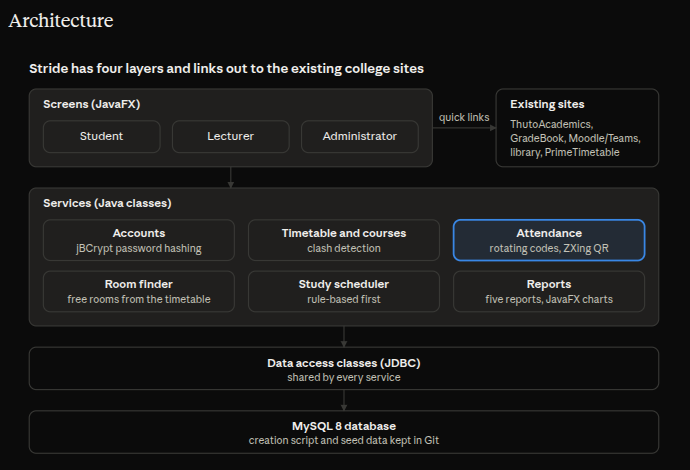
\includegraphics[width=0.97\linewidth,height=0.40\textheight,keepaspectratio]{architecture.png}\caption{Stride four-layer architecture and links to existing college sites.}\end{figure}

\section{Use-case model and functional scope}
The use-case model maps each role to its main system interactions. Authentication is the entry point for role-appropriate functionality. Student use cases focus on self-service and campus navigation; lecturer use cases focus on teaching and attendance; administrator use cases focus on configuration and reporting.
\begin{figure}[H]\centering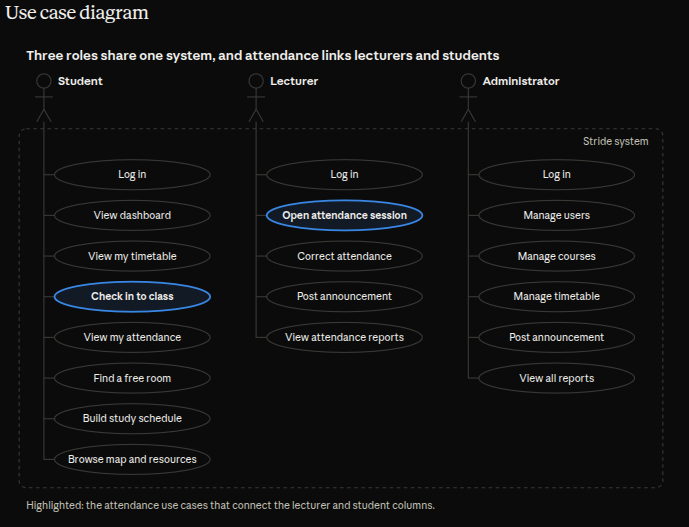
\includegraphics[width=0.98\linewidth,height=0.48\textheight,keepaspectratio]{use_case.png}\caption{Use-case diagram showing Student, Lecturer and Administrator responsibilities.}\end{figure}

\section{Entity relationship diagram (ERD)}
The ERD models the core records required for identity, teaching schedules, campus resources and attendance. \texttt{users} stores account and role information; \texttt{modules} identifies courses/modules and lecturers; \texttt{enrolments} links students to modules; \texttt{rooms} and \texttt{timetable\_entries} represent scheduled teaching and room allocation. \texttt{attendance\_sessions} stores the session code and validity window, while \texttt{check\_ins} records a student's attendance result. Announcements and resources support dashboard content.

The main integrity rule is that a check-in must refer to an attendance session and a student enrolled in the relevant module. Session expiry, session status and duplicate submissions must be checked by the service layer; database constraints should also prevent duplicate check-ins for the same student and session. The diagram is the proposed logical model and should be checked against the final SQL schema before implementation is described as validated.
\begin{figure}[H]\centering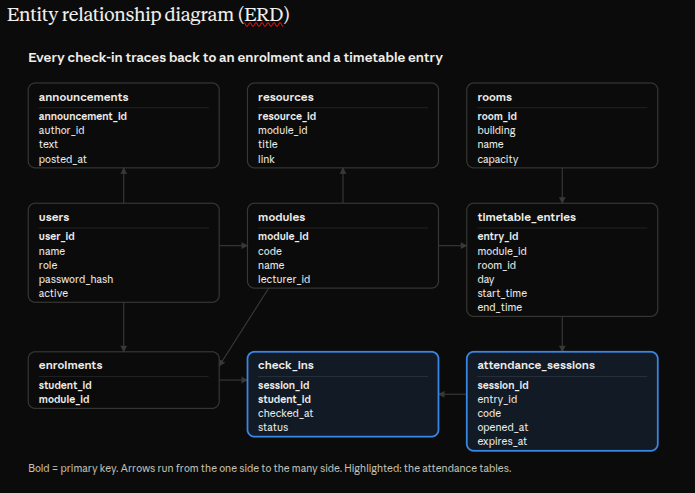
\includegraphics[width=0.97\linewidth,height=0.47\textheight,keepaspectratio]{erd.png}\caption{Proposed ERD showing core entities, keys and relationships.}\end{figure}

\section{UML class diagram}
The class model translates the main domain concepts into object-oriented responsibilities. \texttt{User} is the common account concept, with Student, Lecturer and Administrator specialisations. Module, TimetableEntry and Room model teaching and location data. AttendanceSession represents an active, time-limited class session; CheckIn represents an individual student's attendance event. The operations shown indicate responsibilities such as opening a session, checking a code, validating a check-in, finding a free room and managing reports.
\begin{figure}[H]\centering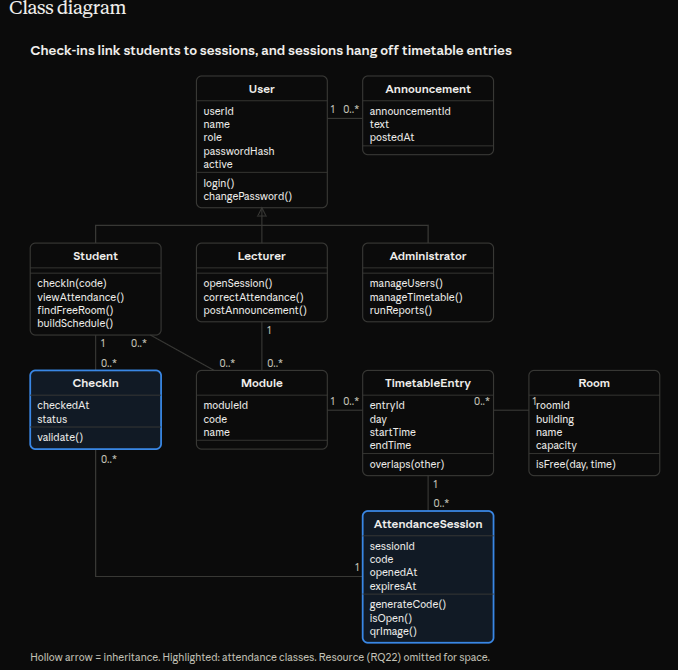
\includegraphics[width=0.96\linewidth,height=0.47\textheight,keepaspectratio]{class_diagram.png}\caption{Domain UML class diagram, including inheritance, operations and multiplicities.}\end{figure}

\section{Attendance check-in sequence}
The sequence model details the key interaction between lecturer, student, Stride and MySQL. A lecturer opens a session; Stride stores the session code and expiry; the student enters the code; and the system validates the code, session and enrolment before saving a check-in. The user receives a confirmation or a rejection reason. The system must not create a valid attendance record when validation fails.
\begin{figure}[H]\centering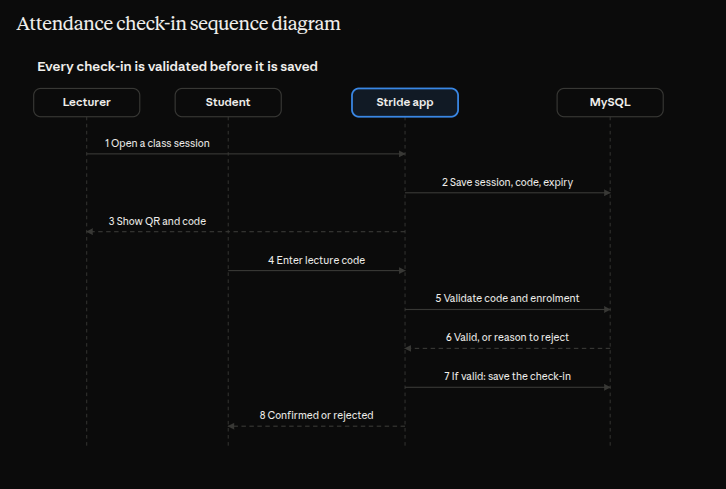
\includegraphics[width=0.96\linewidth,height=0.42\textheight,keepaspectratio]{attendance_sequence.png}\caption{Sequence diagram for attendance session creation and student check-in.}\end{figure}

\section{Dashboard design and implementation approach}
The student dashboard prioritises today's classes and check-in actions, then shows current free rooms, announcements and quick links. Navigation provides access to timetable, attendance, rooms and map, study planner and resources. The lecturer dashboard should emphasise session controls and attendance reports, while the administrator dashboard should emphasise user, course and timetable management. Role-specific views reduce clutter and keep common tasks easy to locate.
\begin{figure}[H]\centering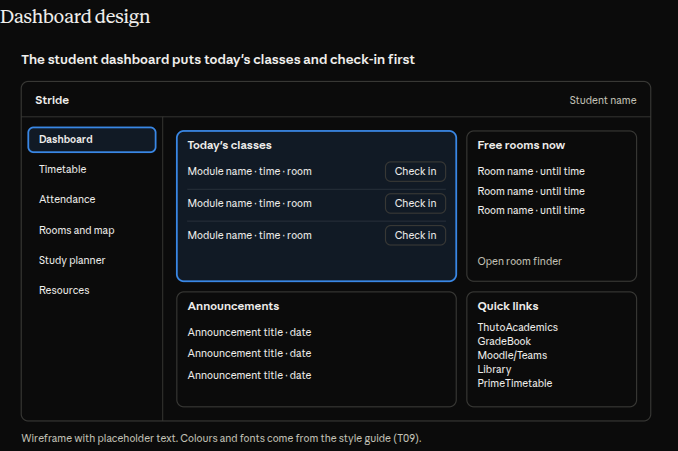
\includegraphics[width=0.98\linewidth,height=0.43\textheight,keepaspectratio]{dashboard.png}\caption{Student dashboard wireframe with sample placeholder data.}\end{figure}

The supplied dashboard is a design prototype, not evidence of a fully connected JavaFX implementation. During development, each panel will be connected through service and JDBC classes, with loading, empty and error states.

\section{Design rules and validation priorities}
\begin{itemize}
  \item \textbf{Access control:} authenticate users and restrict operations by role; never rely on hiding a button alone as authorisation.
  \item \textbf{Attendance integrity:} reject expired or closed sessions, incorrect codes, students not enrolled in the module, and duplicate check-ins.
  \item \textbf{Timetable and room logic:} detect overlapping time intervals; a room is free only when no timetable entry overlaps the requested interval.
  \item \textbf{Database integrity:} define primary and foreign keys, appropriate uniqueness constraints and required fields in the MySQL schema.
  \item \textbf{Model consistency:} align ERD entities and class names with the executed SQL schema and final Java implementation.
\end{itemize}

The immediate validation tasks are to execute the schema in MySQL 8, verify the relationships and constraints, test the attendance success and rejection paths, test room availability against timetable overlaps, and review each dashboard action for the correct role. These are proposed validation activities; no test results are claimed in this design report.

\section*{Conclusion}
The system models describe how Stride's roles, JavaFX screens, service layer, JDBC data access and MySQL records fit together. The ERD establishes the data relationships, the class diagram assigns responsibilities to domain objects, the sequence diagram specifies the attendance flow, and the dashboard wireframe communicates the intended student-facing layout. The next implementation step is to align the diagrams with the executable schema and Java classes, then verify the stated rules through documented tests.
\end{document}
